\documentclass[a4paper, 12pt]{article}
\usepackage[left=2cm,right=2cm,
    top=1.5cm,bottom=2cm,bindingoffset=0cm]{geometry}
\usepackage{cmap}
\linespread{1.5}

\usepackage[T2A]{fontenc}
\usepackage[utf8]{inputenc}
\usepackage{amsmath}
\usepackage{graphicx}
\graphicspath{{pictures/}}
\usepackage{wrapfig}
    \usepackage{caption}


\usepackage{physics}
\DeclareGraphicsExtensions{.pdf,.png,.jpg}
\usepackage[english, russian ]{babel}
\title{ \large \center{Министерство образование и науки Российской Федерации

Федеральное государственное автономное образовательное учреждение высшего образования

"Московский физико-технический институт (государственный университет)"

Физтех-школа ЛФИ

Работа 3.1.3
}

\large \textbf{ Измерение магнитного поля Земли}}
\author{Роман Малов}
\date {19 ноября 2021 г.}
\begin{document}

	\maketitle
\begin{flushleft}
\textbf{Цель работы:} 
определить характеристики шарообразных неодимовых магнитов и, используя законы взаимодействия магнитных моментов с полем, измерить горизонтальную и вертикальную составляющие индукции магнитного поля Земли и магнитное наклонение.
	\end{flushleft}
\ \begin{flushleft}

\textbf{В работе используется:} 12 одинаковых неодимовых магнитных шариков, тонкая нить для изготовления крутильного маятника, медная проволока диаметром (0,5 - 0,6) мм, электронные весы, секундомер, измеритель магнитной индукции АТЕ-8702, штангенциркуль, брусок из немагнитного материала ($25 \times 30 \times 60 \, \text{мм}^3$), деревянная линейка, штатив из немагнитного материала; дополнительные неодимовые магнитные шарики ($ \sim 20$ шт.) и неодимовые магниты в форме параллелепипедов (2 шт.), набор гирь и разновесов.
 \newline
	\end{flushleft}
	\par
\section{Теория}
\textbf{Точечный магнитный диполь} 
Простейший магнитный диполь может быть образован витком с током или постоянным магнитом. По определению, магнитный момент $P_m$ тонкого витка площадью $S$ с током $I$ равен:

 \begin{center}
\begin{equation}
 \vec{P}_{m}=(I / c) \vec{S}=(I / c) S \vec{n}
\end{equation}
\end{center}

где $c$ – скорость света в вакууме, $S = S \vec{n}$ - вектор площади контура, образующий с направлением тока правовинтовую систему,  $\vec{n}$ - единичный вектор нормали к площадке $S$.

Магнитное поле точечного диполя определяется по формуле, аналогичной формуле для поля элементарного электрического диполя: 

 \begin{center}
\begin{equation}
\vec{B}=3\left(\vec{P}_{m} \vec{r}\right) \vec{r} / r^{5}-\vec{P}_{m} / r^{3}
\end{equation}
\end{center}

В магнитном поле с индукцией $\vec{B}$ на точечный магнитный диполь $\vec{P}_{m}$ действует механический момент сил:

 \begin{center}
\begin{equation}
\vec{M}=\vec{P}_{m} \times \vec{B}
\end{equation}
\end{center}
 
 Магнитный диполь в магнитном поле обладает энергией:
  \begin{center}
\begin{equation}
W=-\left(\vec{P}_{m}, \vec{B}\right)
\end{equation}
\end{center}
 
 В неоднородном поле на точечный магнитный диполь, кроме момента сил, действует ещё и сила:
  \begin{center}
\begin{equation}
\vec{F}=\left(\vec{P}_{m}, \vec{\nabla}\right) \vec{B}
\end{equation}
\end{center}

Если магнитные моменты $P_1 = P_2 =P_m$  двух одинаковых небольших магнитов направлены вдоль соединяющей их прямой, а расстояние между ними равно $r$, то магниты взаимодействуют с силой:
  \begin{center}
\begin{equation}
F=P_{m} \partial B / \partial r=P_{m} \partial\left(2 P_{m} / r^{3}\right) / \partial r=-6 P_{m}^{2} / r^{4}
\end{equation}
\end{center}

\textbf{Неодимовые магнитные шары}

Для однородно намагниченного шара намагниченность равна:

  \begin{center}
\begin{equation}
\vec{p}_{m}=\vec{P}_{m} / V
\end{equation}
\end{center}

где $V$ - объём шара.

Индукция магнитного поля $B_p$ на полюсах однородно намагниченного шара связана с величиной намагниченности $p_m$ и остаточной магнитной индукцией $B_r$ формулой:
  \begin{center}
\begin{equation}
\vec{B}_{p}=(8 \pi / 3) \vec{p}_{m}=(2 / 3) \vec{B}_{r}
\end{equation}
\end{center}

\textbf{
Экспериментальное определение величины магнитного момента магнитных шариков} (Метод A).

\begin{figure}[h]
\center{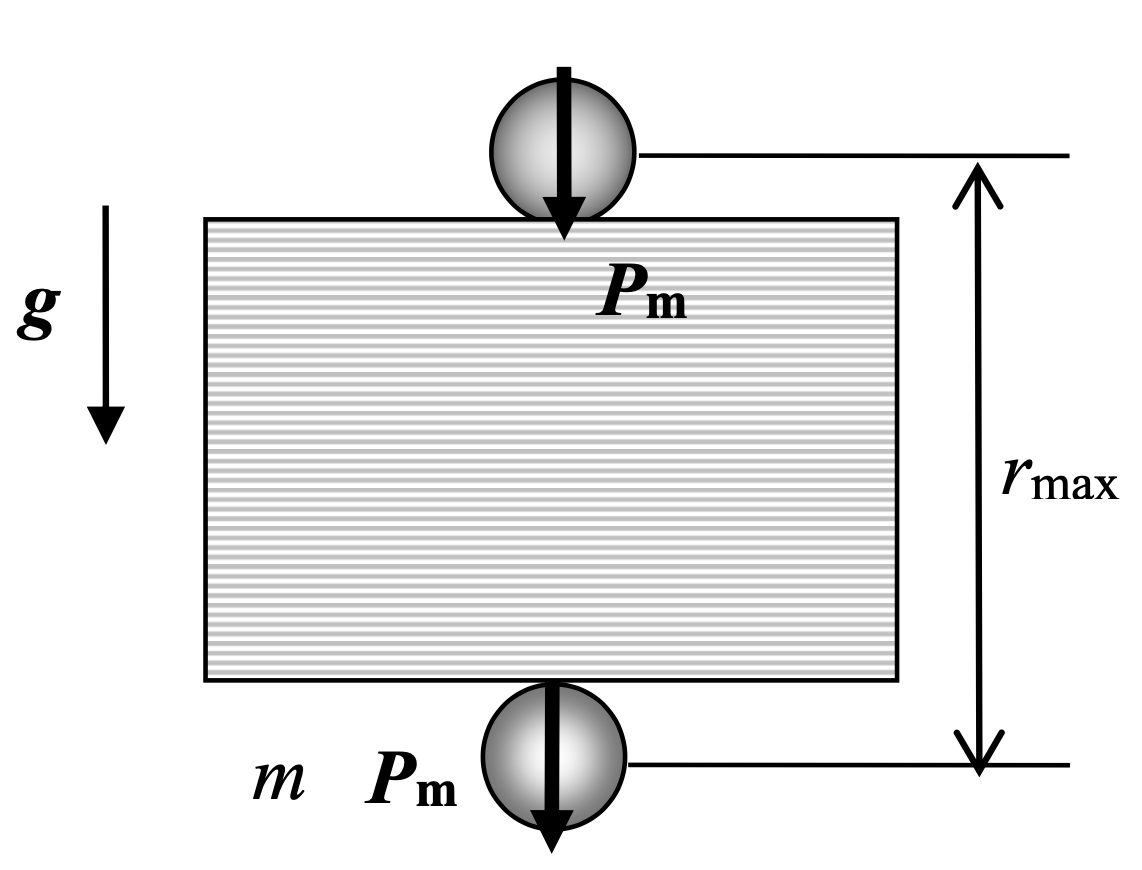
\includegraphics[width=0.9\linewidth]{ris1}}
\caption{Определение магнитного момента шариков по силе тяжести (метод A).}
\label{ris:image}
\end{figure}

Величину магнитного момента $P_m$ одинаковых шариков можно рассчитать, зная их массу $m$ и определив максимальное расстояние $r_{max}$, на котором они ещё удерживают друг друга в поле тяжести (см. рис. 1). При максимальном расстоянии сила тяжести шариков равна силе их магнитного притяжения:

  \begin{center}
\begin{equation}
6 P_{m}^{2} / r_{\max }^{4}=m g, \quad P_{m}=\sqrt{\frac{m g r_{\max }^{4}}{6}}\end{equation}
\end{center}

По величине магнитного момента $P_m$ можно рассчитать величину индукции магнитного поля вблизи любой точки на поверхности шара радиуса $R$. Максимальная величина индукции наблюдаются на полюсах:

  \begin{center}
\begin{equation}
\vec{B}_{p}=2 \vec{P}_{m} / R^{3}
\end{equation}
\end{center}

\textbf{
Определение величины магнитного момента по силе сцепления магнитных шариков} (Метод B).

\begin{wrapfigure}{r}{0.4\textwidth}
\center{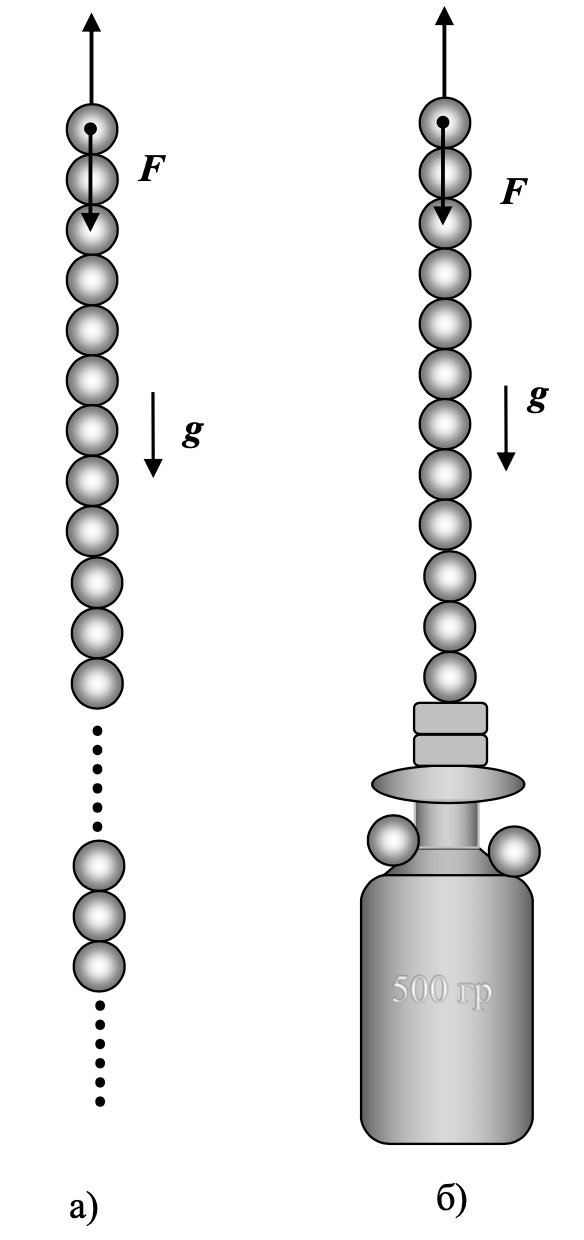
\includegraphics[width=0.9\linewidth]{ris2}}
\caption{Определения магнитного момента шарика по силе сцепления (Метод B).}
\label{ris:image}
\end{wrapfigure}
Величину магнитного момента шариков можно определить также по силе их сцепления. Она определяется как сила, необходимая для разрыва двух сцепившихся магнитных шариков. Сила сцепления максимальна, если шары соединяются своими противоположными полюсами.
Максимальную силу сцепления можно определить по весу магнитной цепочки, которую способен удержать самый верхний магнитный шарик. Если цепь состоит из одинаковых магнитных шариков (см. рис. 2, а), то при определённой длине она 
отрывается от верхнего шарика. При этом, учитывая, что сила притяжения убывает как $r$ в четвёртой степени ($r$— расстояния между центрами шаров) $F \sim 1 / r^{4}$, для расчёта прочности цепочки достаточно учитывать силу взаимодействия верхнего шара с тремя-четырьмя ближайшими соседями.
Если сила сцепления двух одинаковых шаров диаметром $d$ c магнитными моментами $P_m$ равна:

  \begin{center}
\begin{equation}
F_{0}=6 P_{m}^{2} / d^{4}
\end{equation}
\end{center}

то минимальный вес цепочки, при которой она оторвётся от верхнего шарика равен:

  \begin{center}
\begin{equation}
F=6 P_{m}^{2} / d^{4}+6 P_{m}^{2} /(2 d)^{4}+\ldots=F_{0}\left(1+1 / 2^{4}+1 / 3^{4}+1 / 4^{4}+\ldots\right) \approx 1,08 F_{0}
\end{equation}
\end{center}

Таким образом, сила сцепления двух шаров равна:

  \begin{center}
\begin{equation}
F_{0}=F / 1,08
\end{equation}
\end{center}

\textbf{
Измерение горизонтальной составляющей индукции магнитного поля Земли} 
\begin{wrapfigure}{r}{0.4\textwidth}
\center{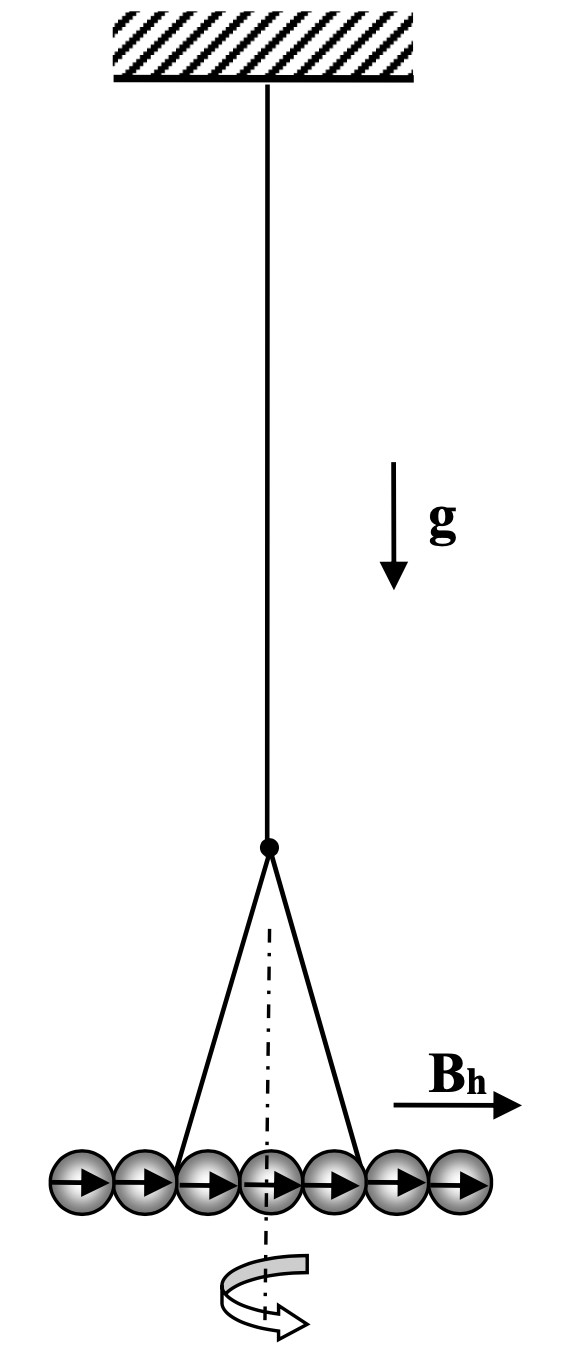
\includegraphics[width=0.9\linewidth]{ris3}}
\caption{Крутильный маятник.}
\label{ris:image}
\end{wrapfigure}
Магнитное поле Земли в настоящей работе определяется по периоду крутильных колебаний магнитной стрелки вокруг вертикальной оси.

"Магнитная стрелка" образована из сцепленных друг с другом противоположными полюсами шариков и с помощью $\Lambda$-образного подвеса подвешена в горизонтальном положении (см. рис. 3). Магнитные моменты шариков направлены в одну сторону вдоль оси "стрелки". Под действием вращательного

момента $\vec{M}=\vec{P} \times \vec{B}$магнитный момент "стрелки" $\vec{P}$ выстроится вдоль горизонтальной составляющей магнитного поля g Земли $\vec{B}_n$ в направлении Юг $\rightarrow$ Север. При отклонении "стрелки" на угол $\theta$ от равновесного положения в горизонтальной плоскости возникают крутильные колебания вокруг вертикальной оси, проходящей через середину стрелки. Если пренебречь упругостью нити, то уравнение крутильных колебаний такого маятника определяется возвращающим моментом сил $M=-P_{0} B_{h} \sin \theta$, действующим на "стрелку" со стороны магнитного поля Земли, и моментом инерции $I_n$ "стрелки" относительно оси вращения.

При малых амплитудах ($\sin \theta \approx \theta$) уравнение колебаний
"стрелки" имеет вид:
  \begin{center}
\begin{equation}
I_{n} d^{2} \theta / d t^{2}=-P_{0} B_{h} \theta, \quad \text { или } \quad I_{n} \ddot{\theta}+P_{0} B_{h} \theta=0
\end{equation}
\end{center}
где $P_0 = n P_m$ — полный магнитный момент магнитной
   "стрелки", составленной из $n$ шариков.
Момент инерции «стрелки», состоящей из $n$ шариков с хорошей точностью равен моменту инерции тонкого однородного стержня массой $m_{\text{ст}}=n m$  и длиной $\ell_{\text{ст}}=n d$:

  \begin{center}
\begin{equation}
I_{n}=(1 / 12) m_{\text{ст}} l_{\text{ст}}^{2}=(1 / 12) n m(n d)^{2}=(1 / 12) n^{3} m d^{2}
\end{equation}
\end{center}

Даже для трёх шариков момент инерции, рассчитанный по приближённой формуле, отличается от точного результата примерно на $2 \%$, а для $n \geq 5$ — различие
не превышает процента; если же учесть, что $T \sim \sqrt{I_{n}},$, то для всех $n \geq 3$погрешность наших расчетов для периода колебаний $T$ не превысит процента, что освобождает нас от необходимости вводить поправочные коэффициенты.

Таким образом, в нашем приближении период колебаний маятника оказывается пропорциональным числу шаров $n$, составляющих «стрелку»:

  \begin{center}
\begin{equation}
T(n)=2 \pi \sqrt{I_{n} / n P_{m} B_{h}}=2 \pi \sqrt{n^{3} m d^{2} / 12 n P_{m} B_{h}}=\pi n \sqrt{m d^{2} / 3 P_{m} B_{h}}=k n
\end{equation}
\end{center}

где $k=\pi \sqrt{m d^{2} / 3 P_{m} B_{h}}$
При выводе этой формулы предполагалось, что магнитный момент — величина аддитивная:
полный магнитный момент системы магнитов («стрелки») равен векторной сумме магнитных моментов шариков, составляющих «стрелку». Экспериментальное подтверждение этой зависимости ($T \sim n$) будет являться косвенным доказательством наших предположений о магнитожёсткости материала магнитов и, соответственно, свойства аддитивности магнитных моментов шаров.

\textbf{Измерение вертикальной составляющей индукции магнитного поля Земли.
Магнитное наклонение.}
\begin{figure}[h]
\center{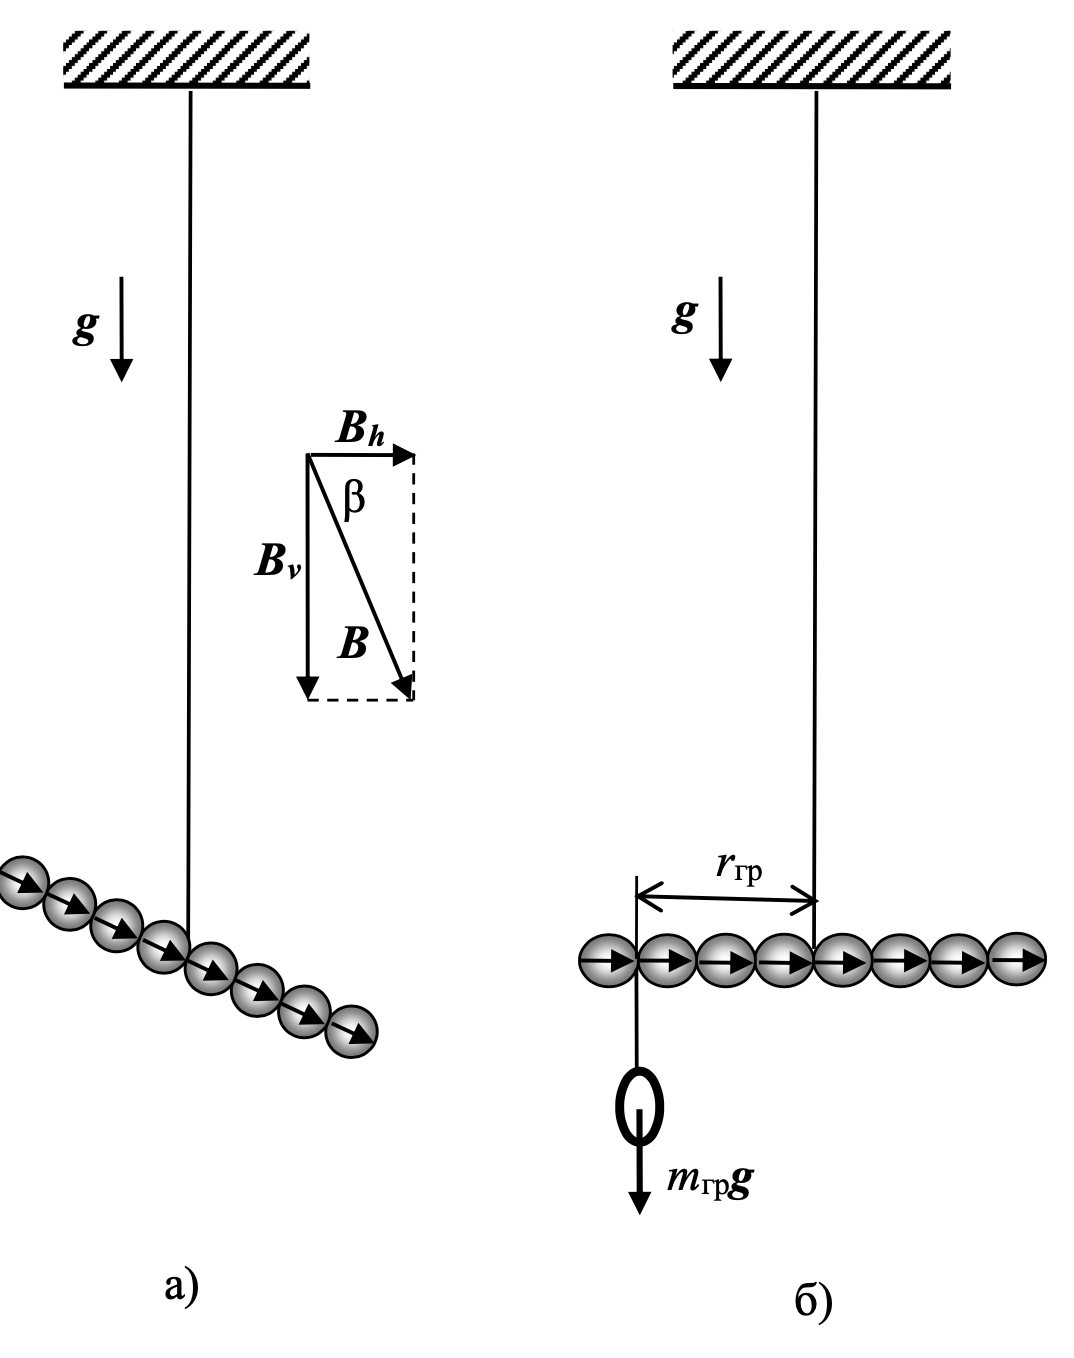
\includegraphics[width=0.4\linewidth]{ris4}}
\caption{Определение вертикальной составляющей поля Земли.}
\label{ris:image}
\end{figure}
Для измерения вертикальной $B_v$ составляющей вектора индукции поля Земли используется та же установка, что и для измерения горизонтальной составляющей с тем лишь отличием, что магнитная «стрелка» подвешивается на нити без $\Lambda$-образного подвеса. В этом случае магнитная «стрелка», составленная из чётного числа шариков и подвешенная на тонкой нити за середину, расположится не горизонтально, а под некоторым, отличным от нуля, углом к горизонту (см. рис. 4, а). Это связано с тем, что вектор $\vec{B}$ индукции магнитного поля Земли в общем случае не горизонтален, а образует с горизонтом угол $\beta$, зависящим от географической широты $\phi$ места, где проводится опыт. Величина угла  $\beta$ называется магнитным наклонением.
С помощью небольшого дополнительного грузика «стрелку» можно «выровнять», расположив её горизонтально (см. рис. 4, б): в этом случае момент силы тяжести груза относительно точки подвеса будет равен моменту сил, действующих на «стрелку» со стороны магнитного поля Земли. Если масса уравновешивающего груза равна $m_{\text{гр}}$ плечо силы тяжести $r_{\text{гр}}$, а полный магнитный момент «стрелки» $P_0 = n P_m$, то в равновесии:

  \begin{center}
\begin{equation}
m_{\Gamma p} g r_{\Gamma p}=P_{0} B_{v}=n P_{m} B_{v}
\end{equation}
\end{center}
($B_v$ — вертикальная составляющая поля Земли). Видно, что момент $M(n)$ силы тяжести уравновешивающего груза пропорционален числу $n$ шариков, образующих магнитную «стрелку»:

  \begin{center}
\begin{equation}
M(n)=A n \text {, где } A=P_{m} B_{v}
\end{equation}
\end{center}

\large{\textbf{Задание № 1}}

\textbf{Определение магнитного момента, намагниченности и остаточной магнитной индукции вещества магнитных шариков}

\large{\textbf{Метод A}}

\begin{enumerate}
\item
Взвесим шарики на весах. Чтобы магнитное поле не повлияло, добавим между шариками и весами толстый слой бумаги. Чтобы убедиться, что магнитное поле не влияет, добавим еще бумаги, и увидим, что значение на весах не меняется.
$M_\text{ш}$ = 39.43 г, $\Delta M_\text{ш} = 0.01 $ г, $L = 27.5$ см, $\Delta L = 0.2$ см, $N = 47$
$m_\text{ш} = \dfrac{M_\text{ш}}{N} = (0.839\pm0.001)$ г, $d=(0.585\pm0.004)$ см
\item


Для начала заметим, что когда прибор для измерения $r_{max}$ показывает ноль, все равно остается небольшой зазор между шариками. 

\begin{figure}[h]
\center{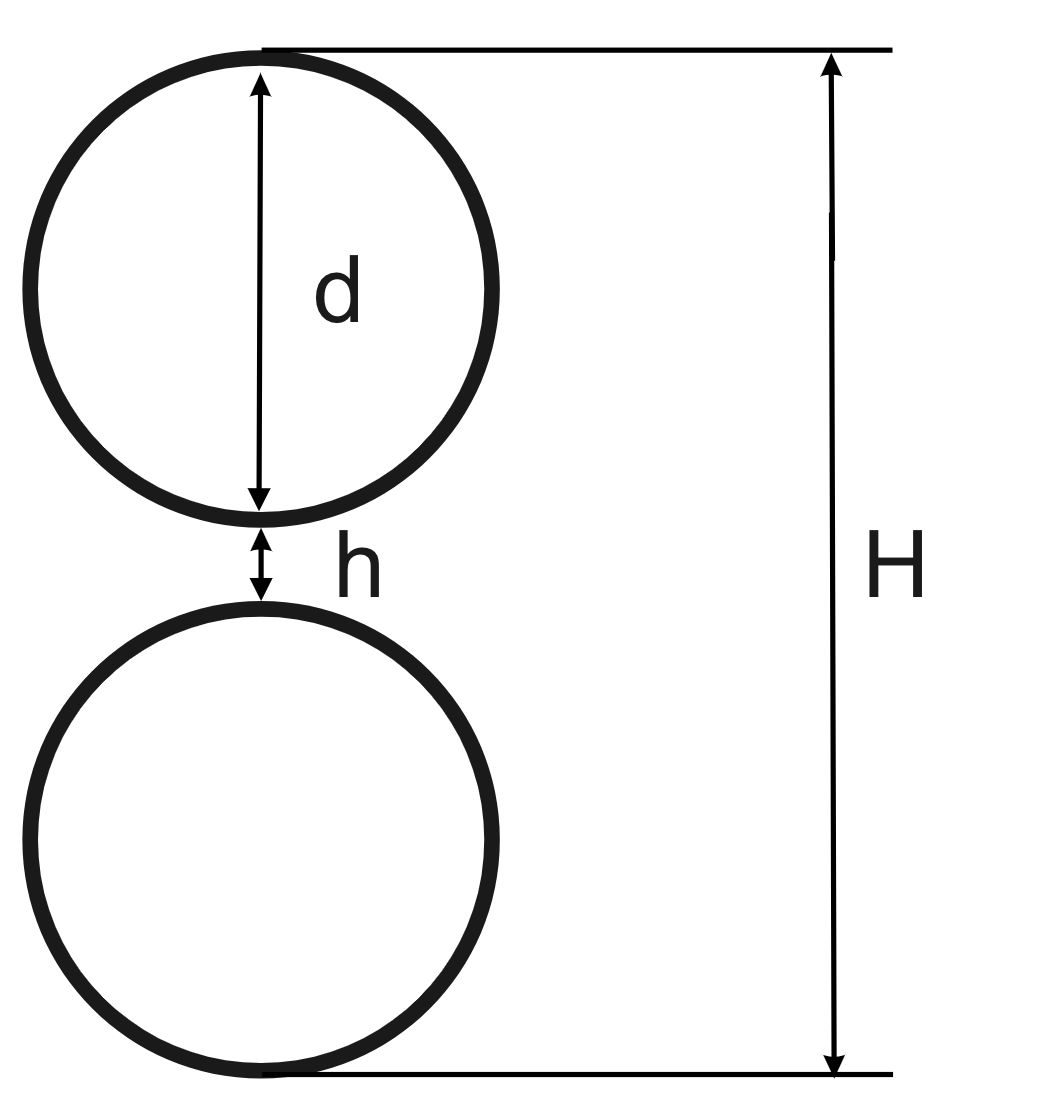
\includegraphics[width=0.4\linewidth]{ris5}}
\caption{Измерение зазора h}
\label{ris:image}
\end{figure}
 Его можно измерить, измерив микрометром расстояние между верхним краем верхнего шарика, и нижнем краем нижнего шарика. $H = (1.271\pm0.005)$ см, $h = H - 2d = (0.101\pm0.007)$ см 

Учитывая зазоры и диаметр шарика, для двух шариков $r_{max} = (2.49\pm0.01)$ см. ($g=980$ гал)

Отсюда $P_m = \sqrt{\dfrac{m_\text{ш} g r_{max}^4}{6}} = (72\pm2)$ эрг/Гс

Но есть возможность, что намагниченности не коаксиальны, и чтобы это исправить, можно поставить сверху 2 магнита и ориентировать их строго вертикально. При этом получаем $r_{max} = (2.72\pm0.01)$  см. В таком случае сила равна $F = 6 P_{m}^{2} / r_{max}^{4} + 6 P_{m}^{2} /( r_{max}+d)^{4}$

Отсюда $P_m = \sqrt{\dfrac{m_\text{ш} g}{6(r_{max}^{-4}+( r_{max}+d)^{-4})}} = (72\pm2)$ эрг/Гс

Видимо, и в первом случае намагниченности были коаксиальны.
\item
Рассчитаем намагниченность материала шариков: 

$p_m = P_m/V =3 P_m/(\pi d^3) = (346\pm11)$ эрг/(Гс$\cdot \text{см}^3)$
\item
Рассчитаем значение магнитного поля на полюсе:

$B_{p}=(8 \pi / 3) {p}_{m}=(2.9\pm0.1)$ кГс

Теперь измерим $B_p$ с помощью магнетометра АТЕ-8702. Получаем $B_p = (3.00\pm0.16)$ кГс.

Результаты совпадают в пределах погрешности.
\item
Рассчитаем величину остаточной магнитной индукции материала, из которого изготовлен магнитный шарик. $B_r = 4 \pi p_m = (4.35\pm0.15)$ кГс

Сравним наш результат с табличными значениями $B_r$ для соединения неодим-железо-бор. В справочнике ГОСТ Р 52956— 2008 она лежит в пределах (9.4 - 14.0) кГс. Мы получили значение меньше, чем справочное. Это можно обьяснить постепенным размагничниванием, которое вызвано механическими воздействиями на шарики.

\large{\textbf{Метод B}}
\item 
Составим цепочку, в которой сначала идут все 47 шариков, потом неодимовые магниты в форме параллелепипедов подсоедините цепочку к гире и разнове- сам, так, чтобы общая масса системы составила ~ 500 г (рис. 2. б). Добавляя или удаляя шарики (шарики можно примагничивать непосредственно к гире), подберите минимальный вес $F$ системы цепочки с гирей, при котором она отрывается от верхнего шарика.
\item
Взвесим всю цепочку. Получаем $F = (273\pm5)$ кдин
\item
Сила сцепления двух шаров: $F_0 = F/1.08 = (252\pm5)$ кдин.
\item
Из формулы $F_{0}=6 P_{m}^{2} / d^{4}$ получаем $P_m = \sqrt{F_0 d^4/6} = (70\pm3)$ эрг/Гс. Здесь учтено, что погрешность поправочного коэффициента 1.08 не больше 1 процента.
\item
Поле на полюсах $B_{p}=(8 \pi / 3) {p}_{m}=(2.8\pm0.2)$ кГс, совпадает с измеренным магнитометром в пределах погрешности.
\item
Метод А дает более точный результат, т.к. его погрешность меньше

\large{\textbf{Задание № 2}}

\textbf{Определение горизонтальной составляющей магнитного поля Земли}

\item Соберем крутильный маятник и, используя $\Lambda$-образный подвес, установим «магнитную стрелку» из 12 магнитных шариков в горизонтальном положении (юстировка системы).

\begin{minipage}{.49\textwidth}
  \centering

\center{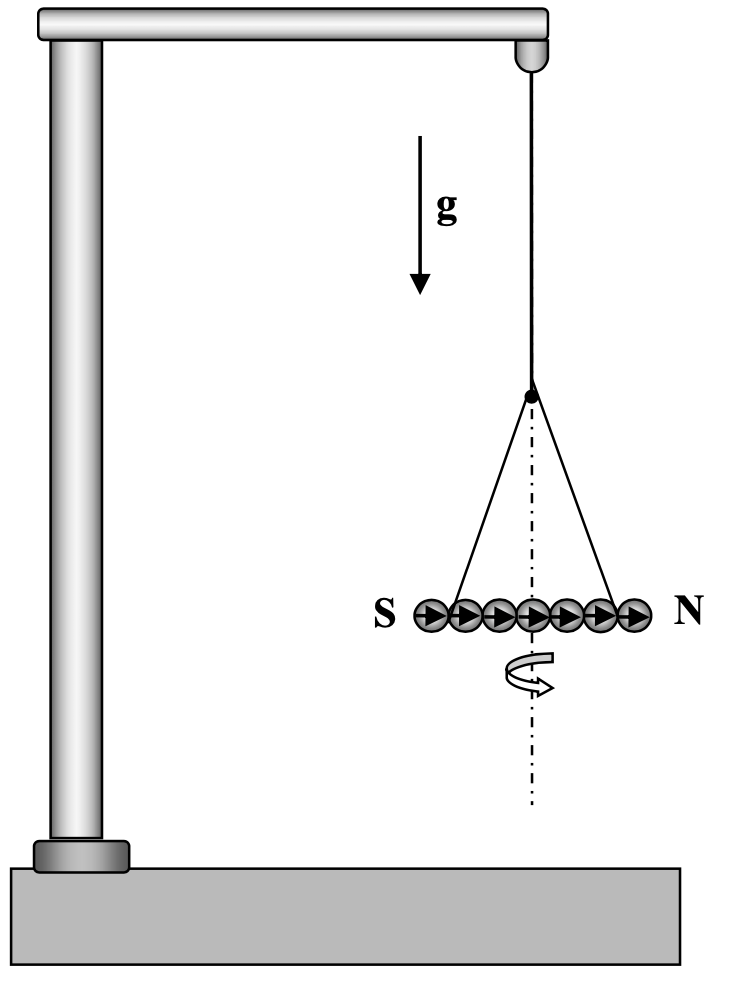
\includegraphics[width=0.85\linewidth]{ris6}}
  \captionof{figure}{Схема установки для определения горизонтальной составляющей поля Земли.}
\end{minipage}
\begin{minipage}{.49\textwidth}
  \centering

\center{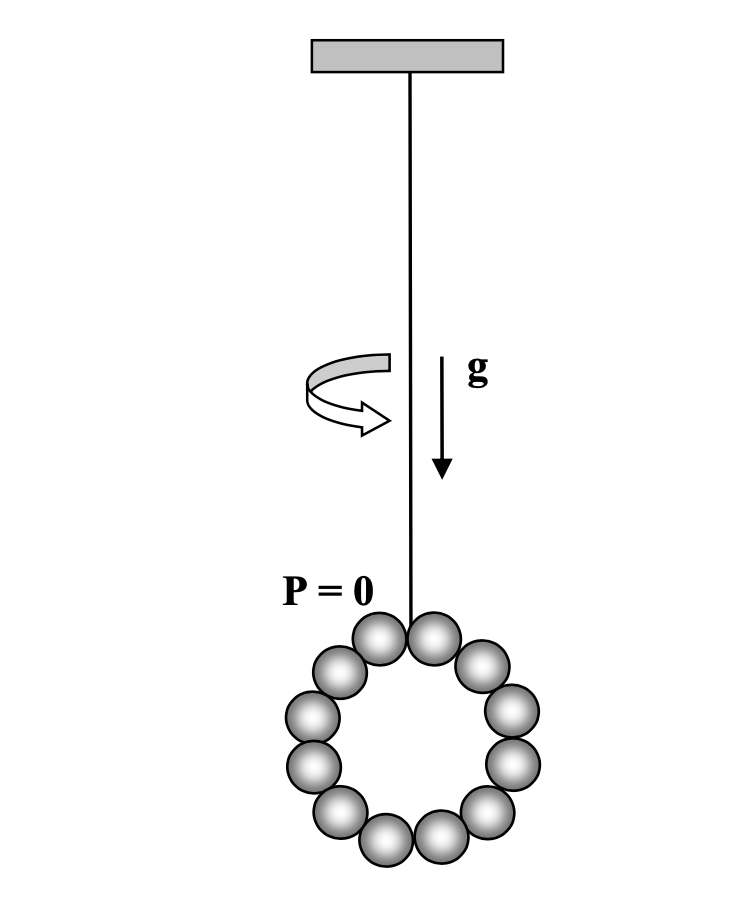
\includegraphics[width=0.85\linewidth]{ris7}}
  \captionof{figure}{Магнитная «стрелка», свёрнутая в кольцо.}
\end{minipage}

\item Покажем, что упругость нити можно не учитывать. Измерим период колебаний кольца. $T \approx 60$ c. Введем эффективный коэффициент упругости нити$\chi$: $I \ddot{\phi} + \chi \phi = 0$. Момент инерции кольца можно оценить как $I=\frac{12 m R^{2}}{2}=6.3 \,\text{г} \cdot \text{см}/\text{с}^2$ 

Т.к. $T = 2\pi \sqrt{\chi/I}$, то $\chi_{\text{нити}} = (2 \pi /T)^2 I \approx 6 \cdot 10^{-2}  \, \text{г}\cdot \text{см}/\text{с}^4$ 

Найдем диапазон $\chi$ у магнитной стрелы. $T_{max} = 3.21$ c, $T_{min} = 0.87$ c, $I_{max} = 41 \,\text{г} \cdot \text{см}/\text{с}^2$,  $I_{min} = 0.7 \,\text{г} \cdot \text{см}/\text{с}^2$

Получаем $\chi_{\text{стрелы}} \in [33, 158] \, \text{г}\cdot \text{см}/\text{с}^4$, что много больше, чем $\chi_{\text{нити}}$, поэтому влияние нити можем не учитывать.

\item
Исследуем зависимость периода $T$ крутильных колебаний стрелки от количества магнитных шариков. Будем отсчитывать 20 колебаний, и записывать в таблицу только период. Время реакции человека $T_{\text{реак}} = 1$ c. $\Delta T = T_{\text{реак}}/20 = 0.05$ c. Данные отображены на таблице 1.


Т а б л и ц а 1
\newline

\begin{tabular}{|l|l|l|l|l|l|l|l|l|l|l|l|}
\hline

T, c & 3.21 & 2.89 & 2.55 & 2.38 & 1.9 & 2.13 & 0.87 & 1.6 & 1.4 & 1.16 \\ \hline
n & 12  & 11 & 10& 9 & 7 & 8 & 3 & 6 & 5 & 4 \\ \hline

\end{tabular}

Построим график $T(n)$ (рис. 8) 
\begin{figure}[h]
\center{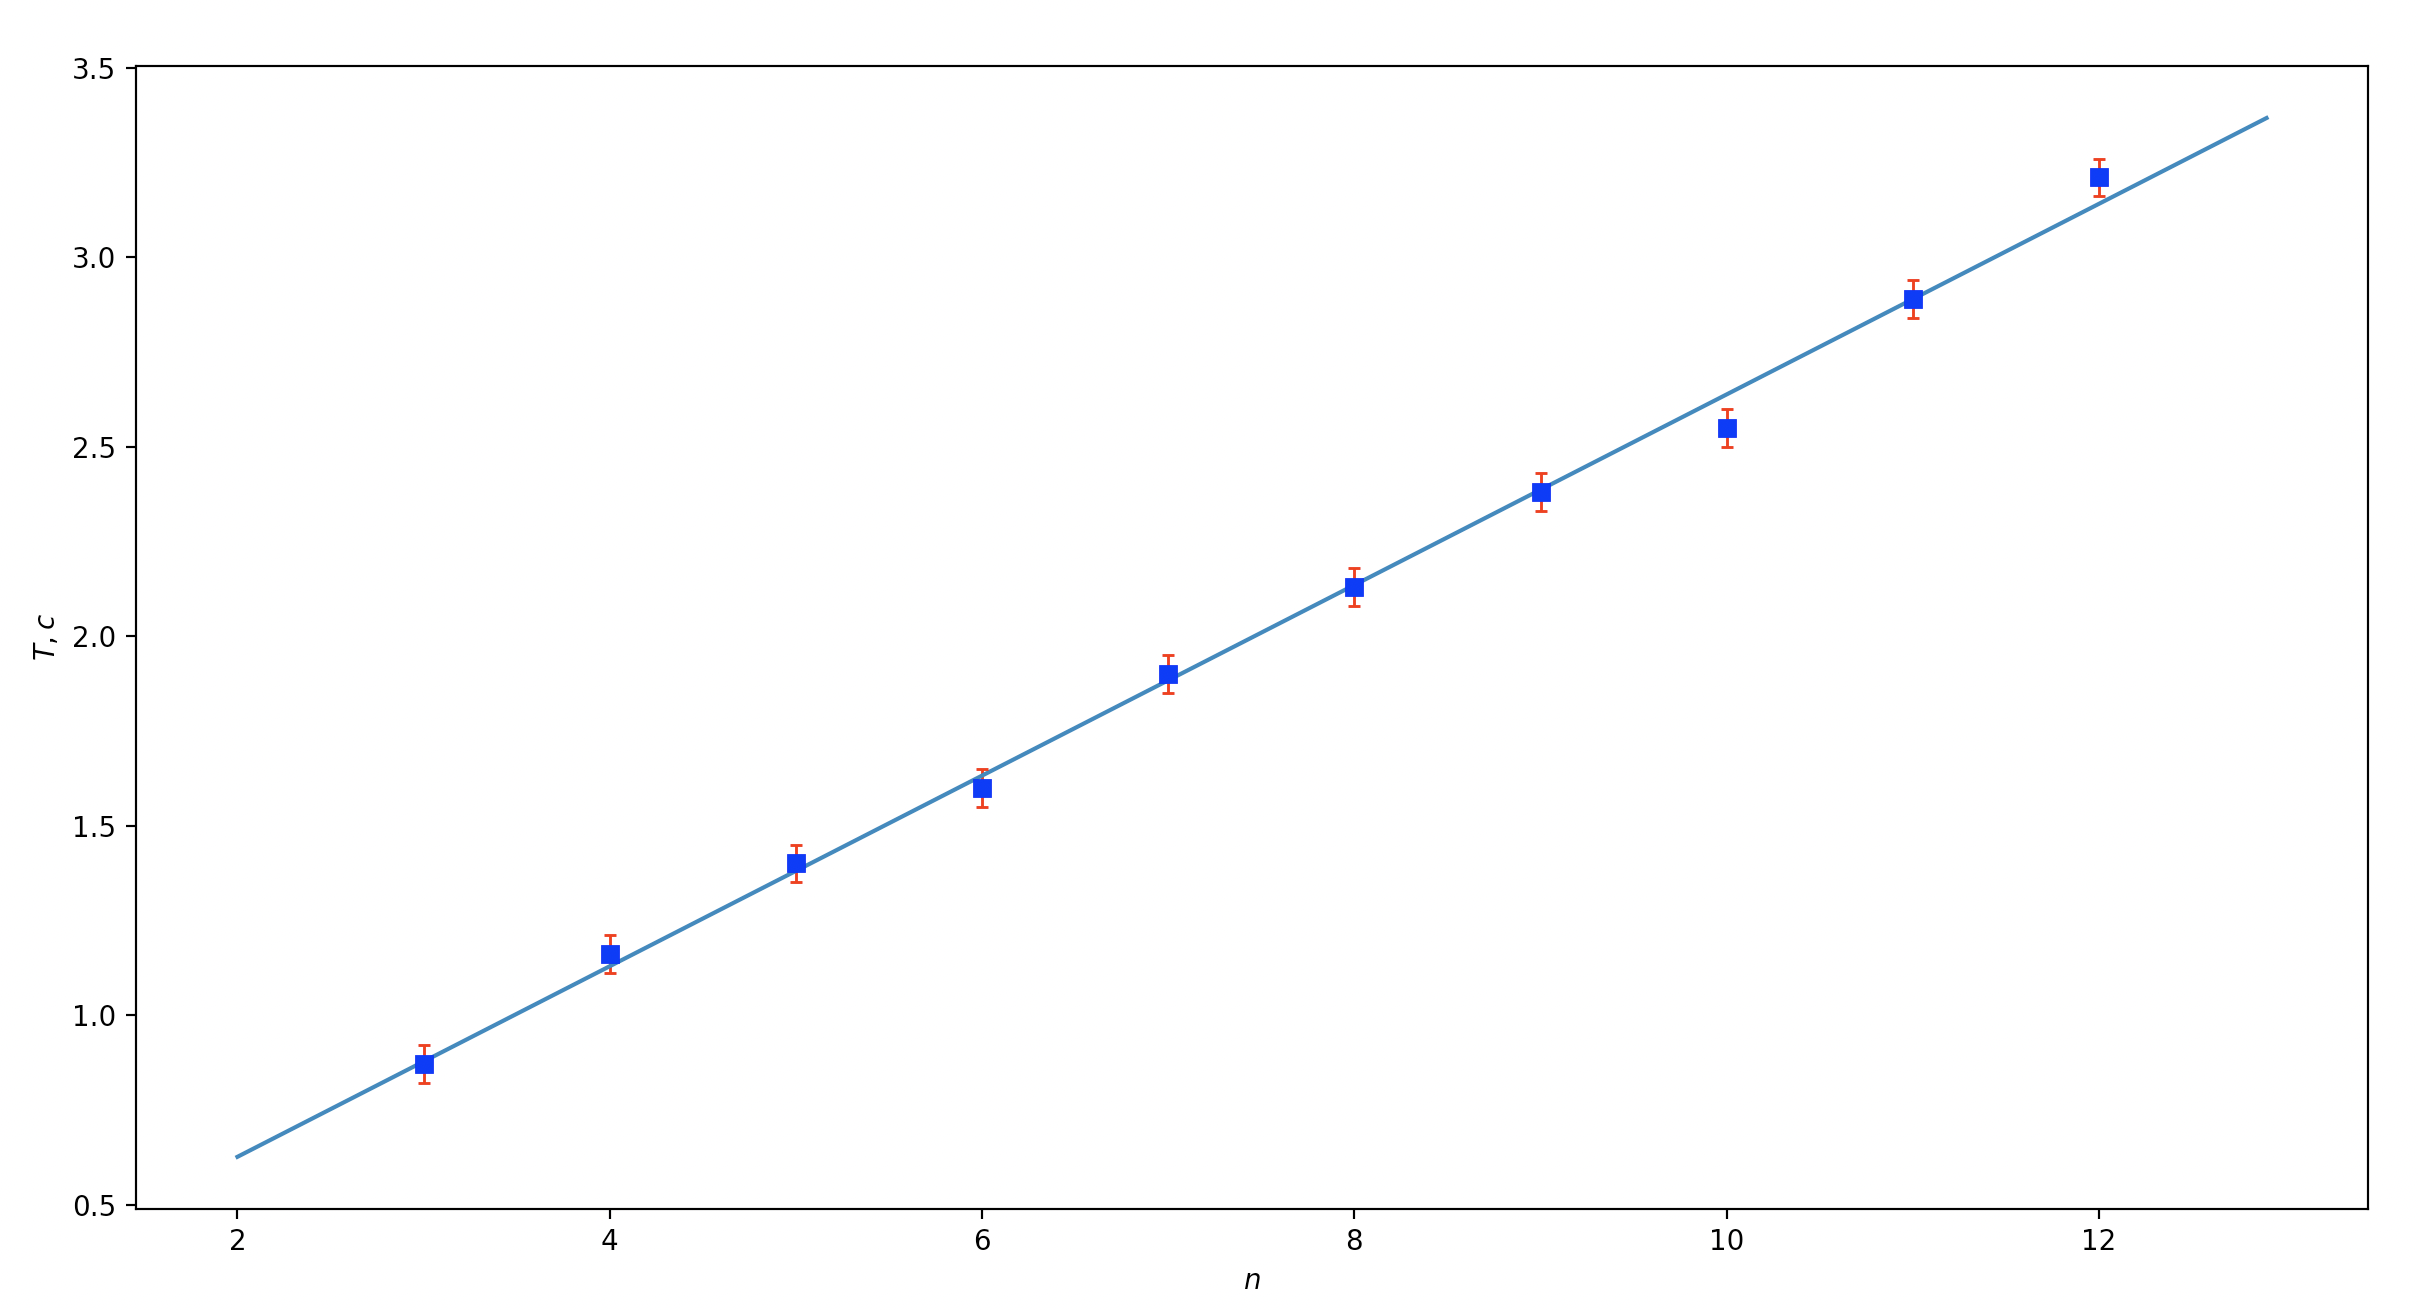
\includegraphics[width=0.9\linewidth]{ris8}}
\caption{График $T(n)$}
\label{ris:image}
\end{figure}
\item
Видим, что график это прямая пропорциональость $T=kn$.
Из МНК получаем коэффициент  $k = (0.251\pm0.007)$ c,  $\chi^2/(10-2) $= 0.76
\item
По значению углового коэффициента $k$ рассчитаем величину горизонтальной составляющей магнитного поля Земли по формуле: $B_{h}=\pi^{2} m d^{2} / (3 k^{2} P_{m}) = (0.207\pm0.013)$ Гс


\textbf{Задание  № 3}

\textbf{Определение вертикальной составляющей магнитного поля Земли}
 \item
 Изготовим магнитную «стрелку» из n = 10 шариков и подвесим её за середину с помощью нити на штативе (см. рис. 4, а).
 \item
 Приведем магнитную стрелку в горизонтальное положение, уравновесив ее с помощью кусочков проволоки. Масса, расстояние до центра и кол-во шариков указано в таблице 2. $\Delta M = 0.03$ г.
 
 Т а б л и ц а 2
\newline

 \begin{tabular}{|l|l|l|l|l|l|l|l|l|l|l|l|}
\hline

M, эрг & 114.6 & 229.3 & 343.0 & 458.6 & 478.2 \\ \hline
l, см & 0.585 & 1.17 & 1.755 & 2.34 & 2.925 \\ \hline
m, г & 0.20 & 0.20 & 0.20 & 0.20 & 0.16 \\ \hline
n & 4 & 6 & 8 & 10 & 12 \\ \hline

\end{tabular}

\item 
Построим график M(n)

\begin{figure}[h]
\center{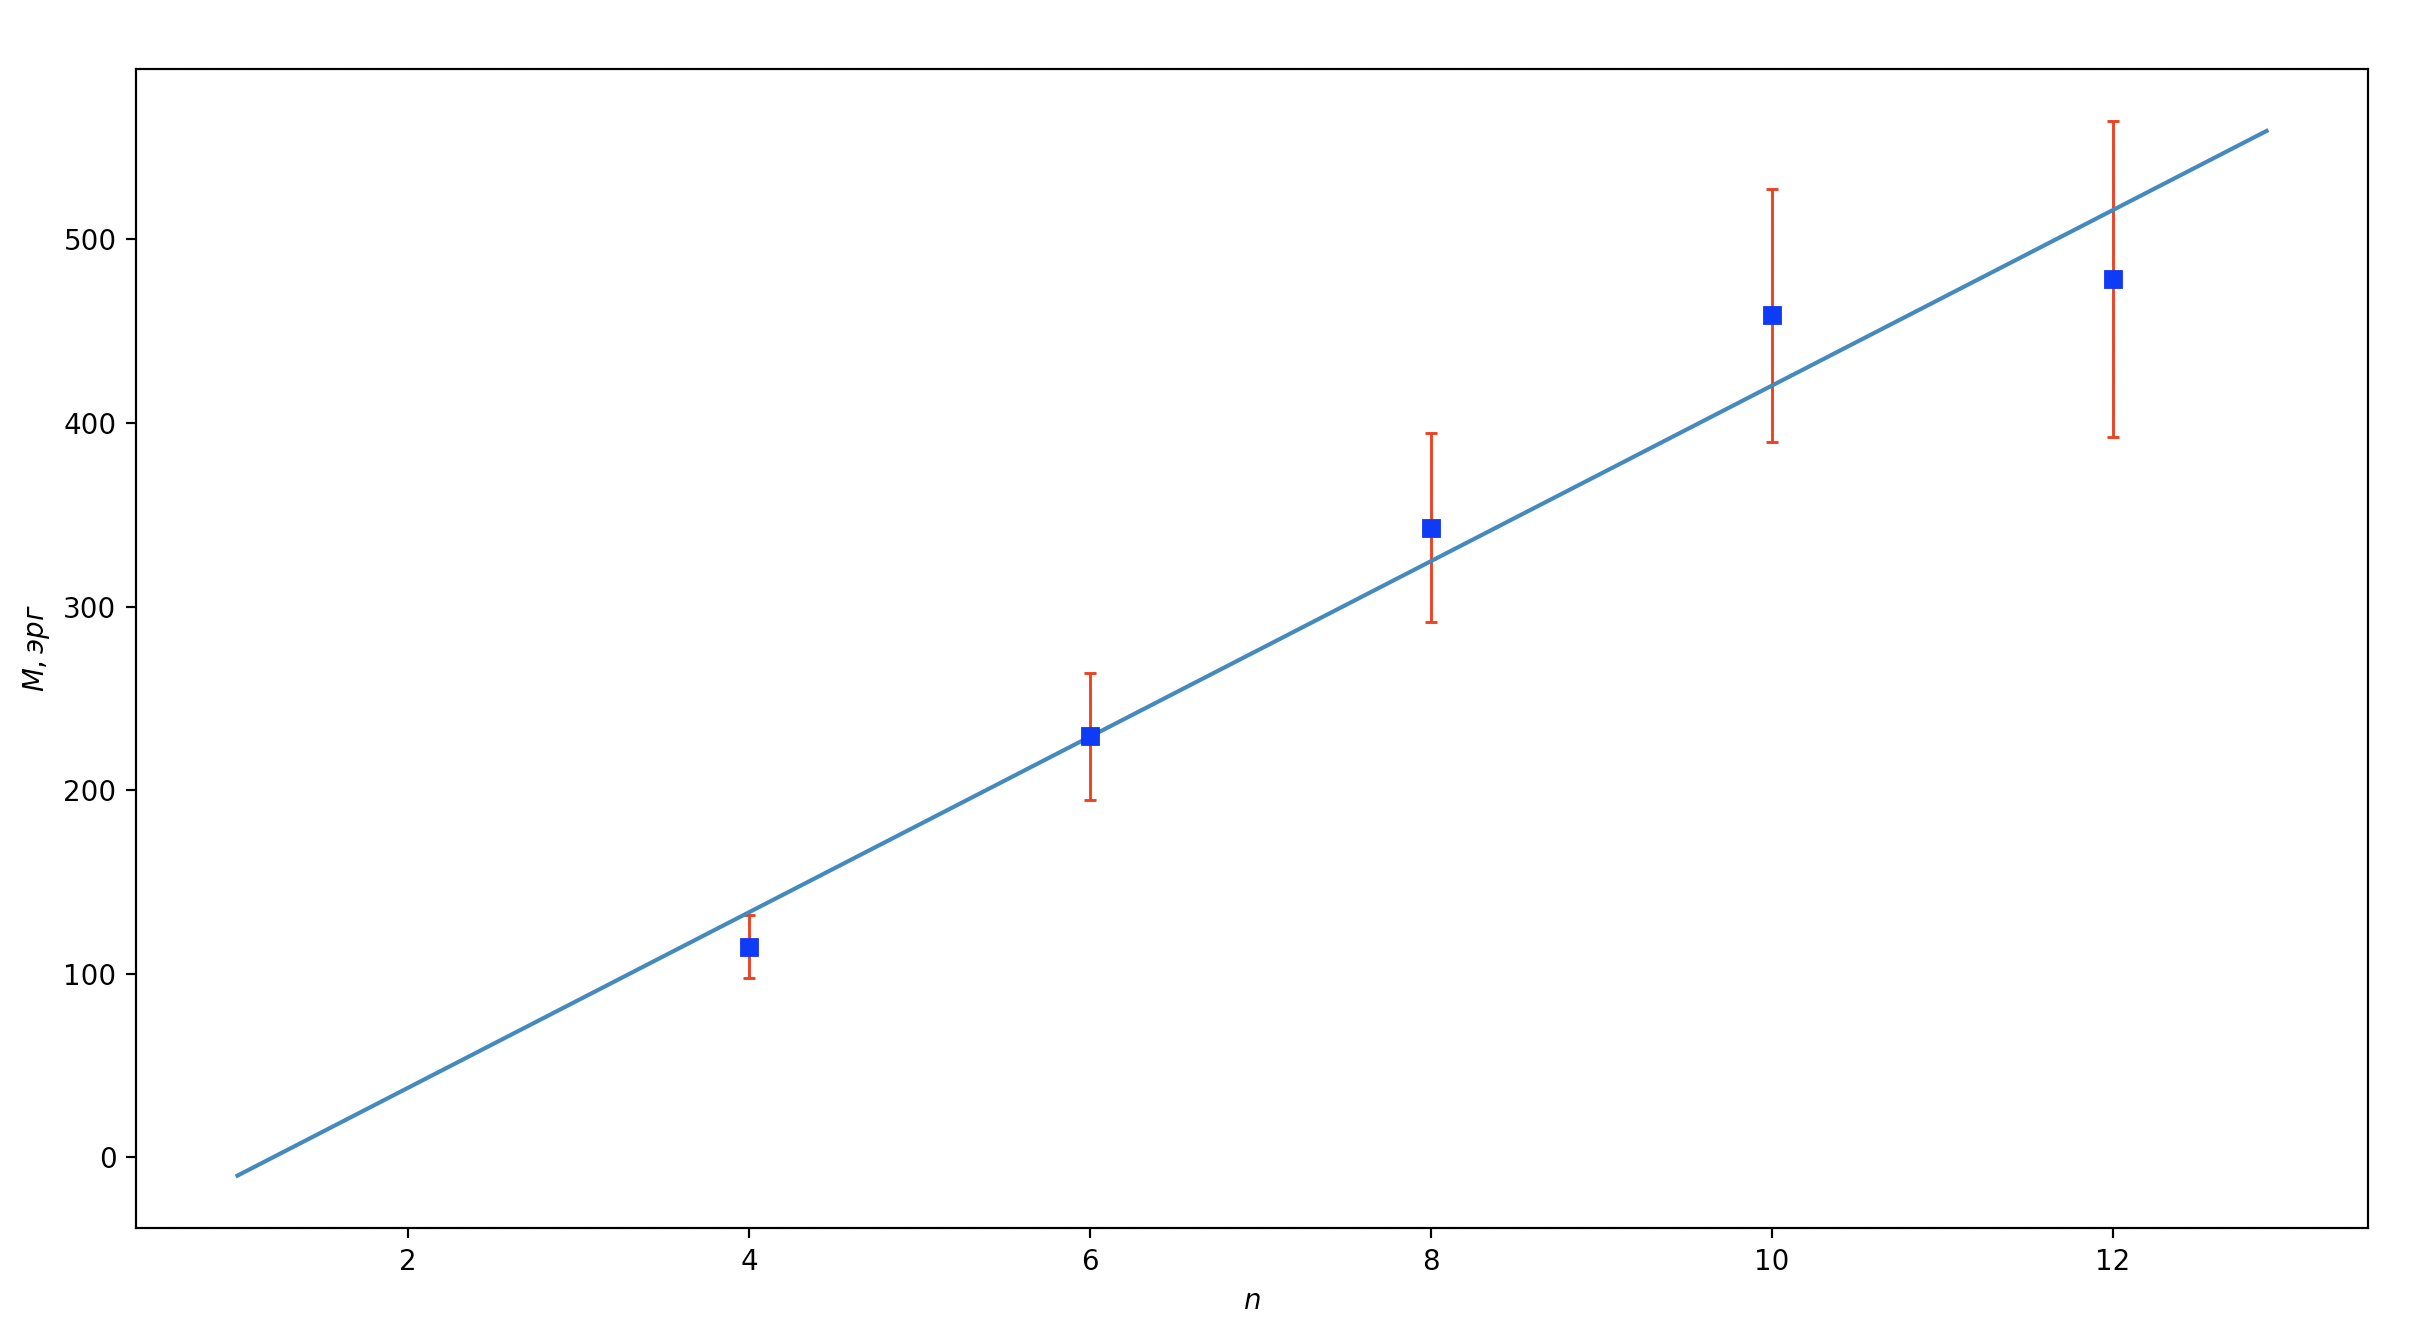
\includegraphics[width=0.9\linewidth]{ris9}}
\caption{График $M(n)$}
\label{ris:image}
\end{figure}
\item

Аппроксимируем график прямой $M = A n$. Мы видим, что точки ложатся на прямую хорошо, поэтому можно считать, что магнитный момент - аддитивная величина.
\item

Из МНК получаем $A = (48\pm6)$ эрг, $\chi^2/(5-2) $= 0.6

Отсюда $B_v = A/P_m = (0.66\pm0.08) $Гс

$\beta = \arctan (B_v/B_h) = (73\pm3)^\circ$

\item


 Пользуясь тем, что индукция $B= P_m/R^3$ и напряженность магнитного $H$ поля внутри сферы однородны, а также граничными условиями $B_{1n} = B_{2n}$ и $H_{1\tau} = H_{2\tau}$ на границе раздела сред воздух/земля. Получаем магнитное наклонение $\vec{B} \, (\phi = 56^\circ$)
 
   \begin{center}
\begin{equation}
\beta=\arctan \frac{\frac{2 P_{m} \cdot \sin \phi}{R^{3}}}{\frac{-P_{m} \cdot \cos \phi}{R^{3}}}=-\arctan (2 \tan \phi)=-71^{\circ}
\end{equation}
\end{center}

\item
Справочные данные: $B_v = 0.5$ Гс, $B_h = 0.15-0.20 Гс$, $\beta = 70^\circ$ (данные взяты из Справочника физических величин под ред. И.С. Григорьева, Е.З. Мейлихова - Москва: Энергоатомиздат, 1991.). Все справочные данные сходятся с измеренными нами в пределах погрешности.


 \end{enumerate}. 

\end{document}